\section{ROS (Robot Operating System)}
\subsection{ROSとは}
ROS(Robot Operating System)とはOpen Source Robotics Foundationによって管理されているソフトウェア開発者のロボット・アプリケーション作成を支援するフレームワークである.
具体的には,ハードウェア抽象化,デバイスドライバ,ライブラリ,視覚化ツール,メッセージ通信,パッケージ管理などが提供されている.\cite{kurazume}.

\refig{ros_topic}に示すようにROSではプロセス(実行プログラム)はノードという単位で扱い,ノード間の通信はトピックと呼ばれる``Publisher/Subscriber''モデルで実現される\cite{ogura}.

これにより,プログラミング言語や通信相手さえ意識することなく簡単にプロセス間通信を実現できる.
つまり,並列分散処理が簡単に実現できるのである.
これは各ノード間のインタフェース,すなわちトピックの名前と型さえ決定すればノードごとに独立して開発を行うことができるという利点でもある.

以上の利点を考慮し,本研究室ではROSがインストール可能なマイコンボードであるRaspberryPi3 Model B上にROSをインストールして開発を進めていくこととした.
\vspace{5mm}

\begin{figure}[htb]
  \centering
    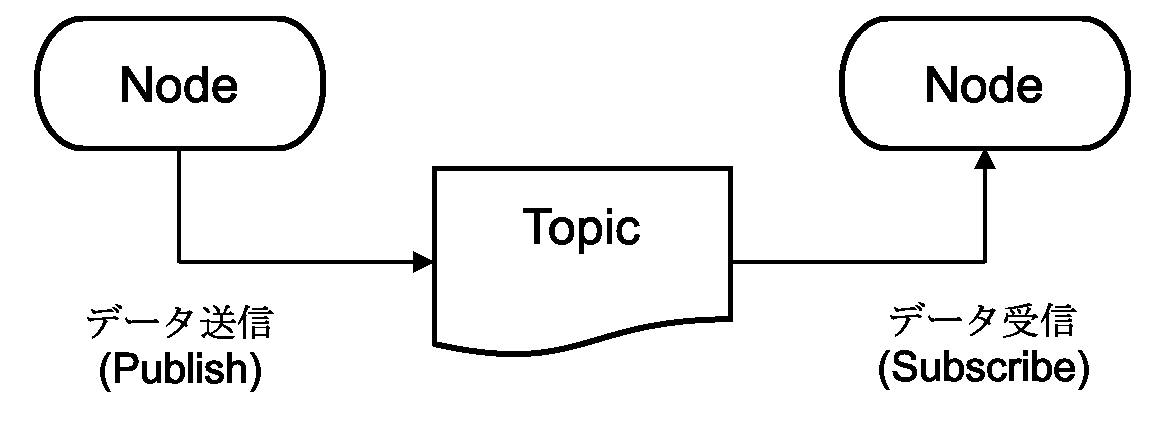
\includegraphics[width=0.5\hsize]{picture/eps/ros_topic.eps}
    \caption{ROSノードとトピックの概念}
    \label{fig::ros_topic}
\end{figure}



\begin{figure}[htb]
  \centering
    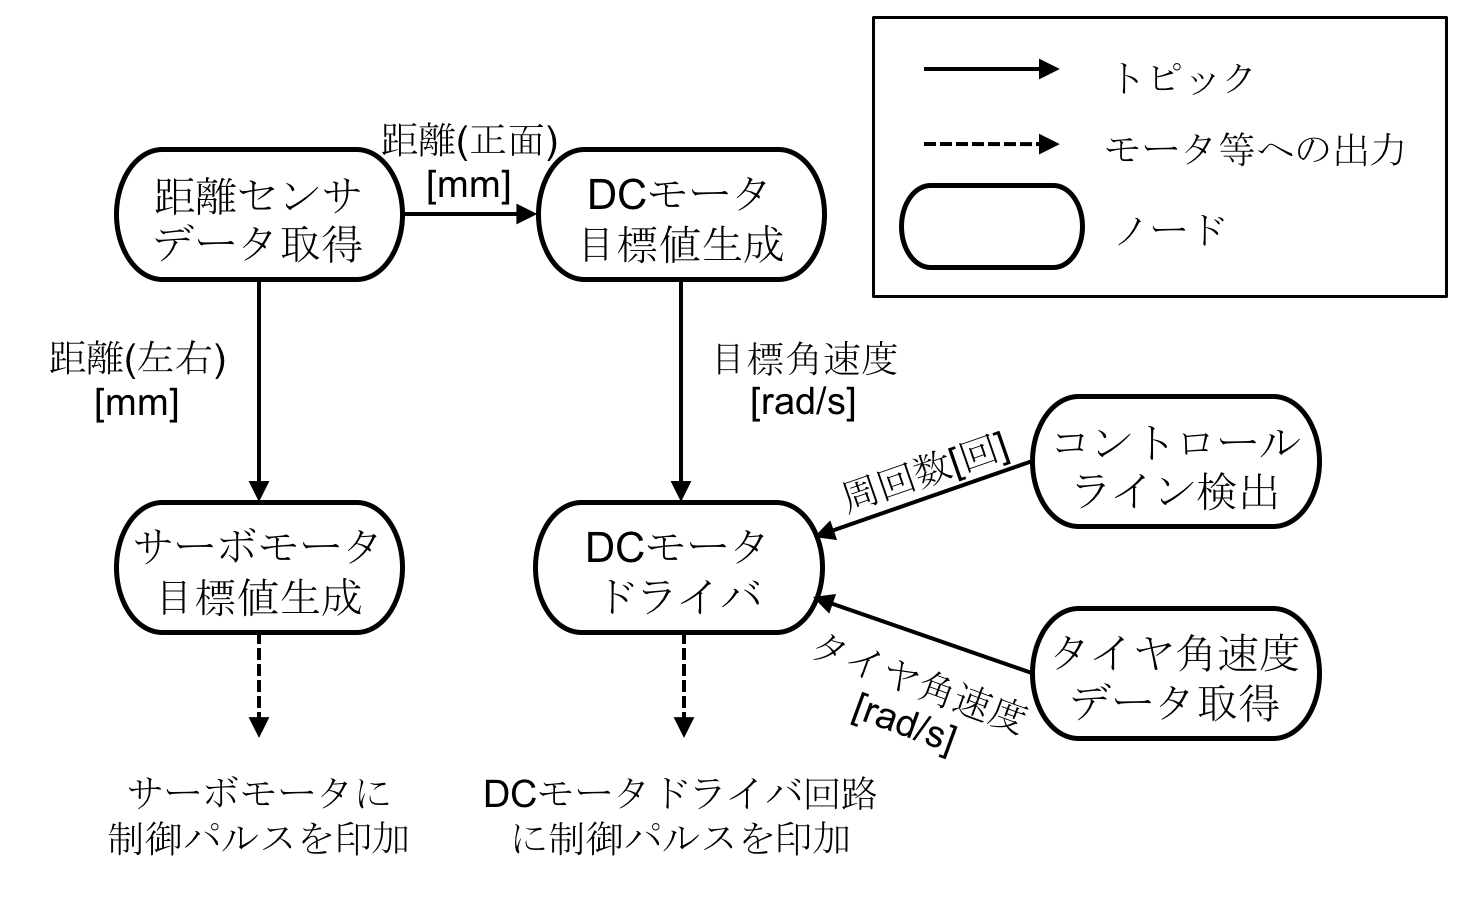
\includegraphics[width=0.8\hsize]{picture/eps/ros_nodes.eps}
    \caption{ROSノードとトピックの構成}
    \label{fig::ros_nodes}
\end{figure}

\newpage
\subsection{ROSノードとトピックの構成}
\refig{ros_nodes}に開発するROSノードとトピックの構成を示す.各ノードの役割は次の通りである.
\begin{description}

    \item[距離センサデータ取得] \mbox{} \\
      ロボカーの前方及び両側面に設置した距離センサからシリアルバス規格の一つである$\mathrm{I^2C}$を介して距離データを$\mathrm{mm}$単位で取得し,外れ値処理や正規化を施した後にPublishする.
    \item[コントロールライン検出] \mbox{} \\
      ロボカーの後方下部に設置したフォトリフレクタによってコントロールラインを通過した回数をカウントしPublishする.

    \item[タイヤ角速度データ取得] \mbox{} \\
      ロボカーの後方に設置したロータリーエンコーダによって計測したタイヤの回転角を基に,タイヤの回転角速度を算出してPublishする.

    \item[DCモータ目標値生成] \mbox{} \\
      ロボカーの前方方向の距離データをSubscribeし,それをもとにDCモータに与える目標値を生成してPublishする.

    \item[ドライバ] \mbox{} \\
      DCモータに与える目標値,ロボカーの両側面の壁との距離,タイヤの角速度,周回数をSubscribeし,サーボモータの目標値を生成して,サーボモータを駆動させる.また,DCモータを目標値に追従するようなPI制御系によって駆動する.さらに,規定の周回数になるとロボカーを停止させる.


  \end{description}
